
\documentclass[12pt,a4paper,oneside,titlepage]{article}
\usepackage[pdftex]{graphicx}
%\usepackage[T1]{fontenc} 
\usepackage[latin1]{inputenc}
\usepackage{amsmath}
\usepackage{amsfonts}
\usepackage{amssymb}
\usepackage{stmaryrd}
\usepackage{listings}
\usepackage{subfig}
\usepackage{float}
\lstset{
  language=java,
  showspaces=false, %Leaves spaces blank
  showstringspaces=false, %Leaves spaces in strings blank
  breaklines=true, %Break lines that are too long
  basicstyle=\footnotesize, %The text style and size of the code
  commentstyle=\footnotesize\it, %The text style and size of the code
  extendedchars=true, %Includes danish characters
  numbers = left, %Shows linenumbers
  stepnumber = 1, %The interval with which linenumbers are displayed
  numberstyle=\footnotesize, %The label size
  tabsize = 3, %Breden af tab, default = 8
  linewidth = \textwidth %Liniebreden
}

\floatstyle{ruled}
\newfloat{program}{thp}{lop}
\floatname{program}{Program}

\usepackage[usenames,dvipsnames]{color} % predefined color: http://www.sci.usq.edu.au/staff/robertsa/LaTeX/ltxusecol.html
%\usepackage{cite}
%
\begin{document}
\begin{titlepage}
\begin{center}
\begin{large}
\textbf{\textit{Technical University of Denmark}}\\
\vspace{0.2cm}
\textit{Department of Informatics and Mathematical Modelling}
\end{large}
\vspace{1.5cm}
\hrule height 1.5pt
\vspace{1.0cm}
\begin{large}
02825 Introduction to Computer Game Prototyping
\end{large}
\\
\vspace{0.2cm}
Fall term 2009\\
\vspace{1.0cm}
\hrule height 1.5pt
\vspace{1.5cm}
\begin{Huge}
In the name of Science\\
\end{Huge}
\vspace{7cm}
\begin{normalsize}
$\overline{\text{David Emil Lemvigh s042899}}\hspace*{3cm}\overline{\text{Andreas M�ller s042809}}$\\

\vspace{2cm}
December 15, 2009
\end{normalsize}
\end{center}
\end{titlepage}

\newcommand{\TODO}[1]{\textbf{\textcolor{red}{#1}}}
\newcommand{\uppaal}{\textsc{Uppaal}}
\newcommand{\lejos}{LeJOS}
\newcommand{\rcx}{\textsc{RCX}}
\newcommand{\verify}[1]{\begin{center}{\texttt{#1}}\end{center}}
\newcommand{\source}[1]{\subsection{#1}\lstinputlisting{src/uppaal/#1}}
\newcommand{\sem}[1]{\lceil #1 \rceil}
\newcommand{\semchop}[1]{\lceil #1 \rceil^\smallfrown}

\tableofcontents

%!TEX root = /Users/andreasmller/Documents/DTU/Computerspil/scienceman/report/report.tex
\section{Introduction}
intro
"In the name of science " is a 2d platform action game. The game is centered around the implementation of the chipmunk 2d physics engine. This provides a simulation based gameplay that is both fun and versatile, as the player uses the environment to defeat his enemies instead of  the traditional handgun / assaultrifle/ RPG-lazerplasmablaster. In this report we discuss the concept and vision of the game, along with the implementation of a proof-of-concept prototype, and an analysis of the functionality and playability of the game.  
%!TEX root = /Users/andreasmller/Documents/DTU/Computerspil/scienceman/report/report.tex
\section{In the name of science} % (fold)
In the game you play a scientist who works on a top secret project for a large private corporation. In his work he has developed a pair of gloves, that grands the user various telekinetic abilities.
    When our hero discovers that the corporation he works for plans to use his inventions for various evil deeds, he steals the gadgets, and embarks on a journey to destroy the evil corporation.

The game has two types of characters:
	The hero, who will be unarmed, but equipped with the powergloves.
	The bad guys, consisting of the evil corporations security personel, who will be armed with various weapons, and will try to stop the hero at all cost. 
	Besides from the characters the levels will be populated by a large amount of inanimate objects which both serves as obstacles for the player to pass, and weapons to defeat the bad guys.
	
	
	
     

\subsection{Game rules} % (fold)

The purpose of the game is to eliminate the bad guys and escape the facility.

The hero defeats his opponents by causing a collision between an enemy and an object. This can either be done by accelerating an object into an enemy, or an enemy into an object. The enemy will take damage based on the impact of the collision. Each enemy has a certain amount of health, and each impact will do damage based on the impulse of the impact.
The hero can manipulate objects by using the powers of his powergloves.
\begin{itemize}
	\item PUSH! Push enemies and object away from you with great force causing great damage upon collision.
	\item PULL! Pull objects or enemies towards you.
	\item GRAVITY WELL! The gravity well creates a point in front of the hero with a high gravitational pull. The gravity well pulls nearby objects towards it to create a cluster, which can be used as a shield, or pushed towards an opponent. The gravity well can only be maintained for a short while, and causes the gloves to heat up very quickly.
	\item SLOW! The hero can slow down time, giving him super fast reactions.       	
\end{itemize}

There will be several kinds of enemies trying to stop the player from escaping. 
Some enemies will have ranged weapons and shoot at the player, and some will be armed with melee weapons, and try to attack the player up close. The different enemies, and different combination of enemies will force the player to use different strategies. Hiding behind a couple of crates might work great against a ranged attacker, but the melee enemies will be able to get past them and attack you.

The hero has a health bar which shows how much damage he has taken. The different types of attacks, from the different enemies cause different amounts of damage.

	Each level is divided into sections, and after each section a portion of the heroes health will regenerate. 

	Upon death the hero will return to the start of the section with full health. This way the game player will not continuously be punished by entering a section while low on health.
	
	Heat is generated when the hero uses his gadgets. This is serves as a way to limit his abilities. If his gadgets overheat, they will become temporarily disabled, until they cool down to safe levels.


\subsection{Desired features} % (fold)
desired features

 The game centers around the use of the 2d physics engine, and the ability to use the various objects in a level as weapons. The main features of  the game is therefore the abilities, granted by the powergloves, to manipulate objects.  These abilities must function smoothly, as they are the foundation of almost all aspects of the game.

\paragraph{Puzzles} % (fold)
Besides the combat , the game should include a number of different puzzles that requires the abilities of the powergloves to solve. These can range from obstacles that need to be moved, to ledges that can only be reached by piling crates, or hidden doors that are opened by the PULL! power.

\paragraph{Bossevents} % (fold)
At the end of each level should be a boss event. This can either be a specifik kind of enemy, with a large amount of hitpoints, and special weaponry, or a large scale puzzle, that requires the use of all the heroes abilities to complete.

 
\paragraph{HUD} % (fold)
The game should have a heads up display, that shows the players hitpoints, game score, and boss hit points during a boss fight.



%!TEX root =/Users/andreasmller/Documents/DTU/Computerspil/scienceman/report/report.tex
\section{Implementation} % (fold)
Incorporation and tweaking of the chipmunk physics engine in a way that provides a solid gameplay takes a huge amount of work, and creating a simulation based game involves an endless amount of unforeseen complications. We have therefore reduced the game prototype to a single level, which focuses on the combat involving physical objects. Our prototype does not include a heads up display, or any type of cut scenes to drive the story forward (it technically does not even include a story). These elements may be complex to design properly, but they are trivial to implement. We have therefore chosen to focus on implementing the physics powers described in section 2. This is where the game differs from all other existing platform games, and this is where the challenges of the implementation lies.
\subsection{Project Structure}

The project structure is based that of the Mr. Fuze game, and some of the features are copied directly from this game.These features include loading levels from image files, and the Camera class, which centers the viewport around the player. The level loading feature makes it very easy to create new levels, and makes any basic image editor into a level editor. This gave us a good IDEA / ALTER structure to work from.

\subsection{Graphics}
The game graphics are very crude and simple, since none of the developers have any creative skills what so ever. We have copied the background and platform textures from a python game name robot toast. The characters are simple stickfigures, which adequately serves as avatars, but are not exactly pleasing to the eye. The crown of the sprite collection is the crates, which comes in two different sizes and colors, and has an unseen level of detail compared to the stickfigures.

\subsection{Physics}

The physics implementation is based on pumunk. All our world objects, which inherits from sprite, also contain a body and shape. Pymunk simulates their movement, and sprites are then moved to the body position, and turned based on the angle. Objects are never directly moved by the program, only by applied forces and impulses.

\subsubsection{Game world}

All non-moving platform, are static polygons with infinite mass and inertia, preventing them from being moved while being part of the physics world. 

\subsubsection{Player movement}

The player is a simple rectangle polygon in the physics world. He has a fairly large mass and infinite inertia. This allows him to be hit by the crates he throws around, and be pushed around by them to some extend. Infinite inertia makes sure he's never knocked over or flipped. Movement is done by applying impulse to his body, but with a limit to his maximum speed. This gives acceleration to his movement, while still having him affected by the momentum of objects he collides with. Jumping is similarly done by applying a lateral impulse, he cannot jump again until he collides with another physics object, to allow him to jump from the top of crates. This is one of the places where a compromise have had to be made, and the implementation doesn't quite feel right yet. At the time of writing any collision anywhere on the player, is adequate to a allow jumping again, which mean a player with a crate on his head, can jump straight up forever. Several solutions present them selfs, our preferred being only allowing a jump after a collision with feet of the player, having a upward normal vector. This solution opens up for a rather interesting move, where the player jumps while above a crate, then force pulls it up to his feet. This could in theory be repeated forever, unless power limitations prevent it. This move can be mimicked under current circumstances, and is a rather difficult move, making it more of a feature than a bug if implemented in such a way. Currently stopping feels somewhat odd, since the player with his high momentum, takes a while to stop on his own with using only friction with the surface.

\subsubsection{Player abilities}

\textbf{Force push / pull}

Force push as expected pushes all objects not nailed down, within and area away from the player, and the force pull vice verca.

\begin{figure}[h]
\begin{center}
 	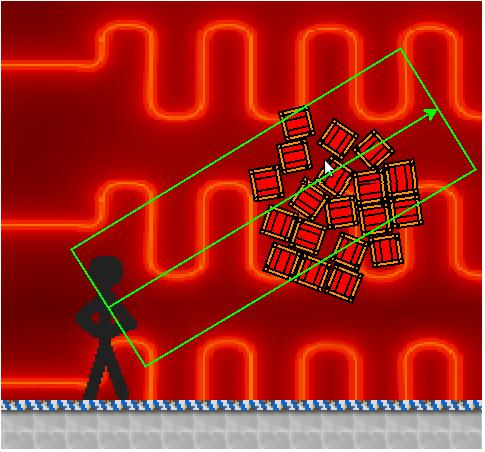
\includegraphics[width=8cm]{pics/push}
	\caption{Force power area of effect}
	\label{fig:force}
\end{center}
\end{figure}

 The power eminates from the player, and is directed towards the current cursor position. These force power have fixed ranges, and all non-static physics objects within the area is applied with a fixed impulse, making smaller object more affected than larger. Both moves can be used aggresively pushing boxes in front of enemies, or pulling crates behind him. But also more creative maneuvers, like pulling crates towards yourself, jumping over them, letting them hit enemies on the other side of the player. 
\\ \\
\textbf{Gravity well}

This power pull all nearby objects towards the cursor. The cursor can be moved, while "holding" object, and can be used in a number of creative ways. The power proved somewhat difficult to implement, and is based on some slightly selfinvented math. The original implementation was to apply a force on all objects within range, which had several problems. All object built quite a large momentum towards the cursor, making them fly almost as far away as they had originally been on the other side of the cursor. Secondly all the objects oscillated horizontally around the cursor.

\begin{figure}[h]
  \begin{center}
 	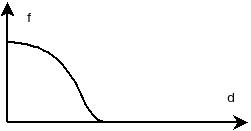
\includegraphics[width=6cm]{pics/force}
	\caption{Force of gravity well based on distance}
	\label{fig:Gravity}
\end{center}
\end{figure}

The final version is have a polyminally growing force towards the cursor, with a cap on the maxiumum force. It also have a velocity dampening of 1\% to avoid oscilation which works quite well.
\\ \\
\textbf{Timestop / Timeslow}

Not all of the abilities planned in the original design document have been implemented. A timestop or timeslow ability was dropped, which originally was planned to be used to enable more complex maneuvers with the physics powers. Things like jumping on crates falling in mid air and dodging enemy bullets. This ability was party dropped due to time constraints, but the game currently doesn't feel like it needs this ability. The higher pace and reaction time give an extra sence of danger, and makes difficult moves feel more rewarding when they succeed. It could have been implemented by reducing the simulating step count, while retaining the pygame tick framerate.


%!TEX root = /Users/andreasmller/Documents/DTU/Computerspil/scienceman/report/report.tex
\section{Analysis} % (fold)

The proof-of-concept prototype allows us to get a feel of how the different powers work, which is the most essential part of the gameplay. It has allowed us to tweak different aspects of the physics objects, in order to give the combat a more fluently feel. 
\subsection{Playability} % (fold)
	After playing the game for a while you realize just how endless the players possibilities are. Since all combat is based on simulation, instead of hardcoded attacks, no two combat scenarios will ever be the same. In fact playing the same encounter over and over will be a new experience every time. 



\subsection{Feedback} % (fold)
We persuaded a few friends to test our game prototype. Our intro level at the time had an enemy placed right next to the players starting point, which caused some problems, since it did not allow the player to become familiar with the game mechanics.  Once the testers were given the time to try out the different powers the tester quickly picked up the game, and went on to crush all the badguys we threw at them. We observed as they found creative ways to kill their enemies, that we had not event thought possible.

Mads Ingwar, one of the testers had this to say:

\quote{"The game starts in-medias-res, which sets you straight in the action. This along with a very aggressive enemy AI makes for quite an action surge straight off the bat.

The game's selling point is the unlimited fun to be had with physic powers. The interaction with the crates work seamlessly, and is very intuitive. It is especially nice that small tricks such as pulling a crate up and then forcepushing it towards the enemy at kill-speed works as expected. Furthermore the gravity well implementation is really nice both visually (some abstraction may apply) and in game terms. 

Overall the game is very addictive and I was soon lacking both enemies and more levels".}


\subsection{Reflection} % (fold)
One thing we constantly observed, was the unpredictability of both the players, and the game it self. The simulation based gameplay combined with the creativity of the players result in an infinite number of solutions to any game situation. An important strategy for the future development of the game will therefore be to avoid limiting the player, and make sure that every problem in the the game can have several solutions. Every level in the game must therefore also serve as a playground for exploring the physics powers.
%!TEX root = /Users/andreasmller/Documents/DTU/Computerspil/scienceman/report/report.tex
\section{Conclusion} % (fold)

\appendix
\include{Source}
\end{document}